\section{Betting on volatility -- around varswaps}

\begin{tcolorbox}[width=\linewidth, sharp corners=all, colback=white!95!black]
    A desk is interested in expressing a view on volatility. To do so they suggest entering a variance swap contract with payoff:
    \[\dfrac{1}{T} \int_{0}^{T} \sigma_t^2 dt - \sigma_K^2\]

    On the sell side, how would you price and hedge such a contract?\newline
    On the buy side, if your goal is to tail-hedge your portfolio, could you suggest other approaches than buying a varswap?

\end{tcolorbox}

Variance swaps are heavily important instruments: while vanilla options reveals the implied density of the underlying at maturity, varswaps give some information about the path the asset will take. These products are also used to construct the forward variance curve which is taken as an input in Bergomi models.

\subsubsection*{Hedging varswaps}
Could we find a smooth transformation of the asset that would help in the replication of the payoff? Applying Itô's formula to $f(S_t)$, we get:
\begin{equation*}
        \resizebox{\hsize}{!}{$ f(S_t) = f(S_0) + \int_0^T f'(S_t) \,dS_t + \dfrac{1}{2} \int_0^T f''(S_t) \,d\langle S_t\rangle = f(S_0) + \int_0^T f'(S_t) \,dS_t + \dfrac{1}{2} \int_0^T f''(S_t) \sigma_t^2 S_t^2 \,dt $}
\end{equation*}


To make the variance swap variable leg appear, remark that taking $f = \log$ indeed yields $f''(x) = x^{-2}$.
This yields:
\[
    \int_{0}^{T} \sigma_t^2 dt = 2 \int_0^T \dfrac{dS_t}{S_t} - 2 \log \dfrac{S_T}{S_0}.
\]

The difficulty here is in the replciation of the log contract. As we are in the case of a twice differentiable payoff $\phi$, we can apply the \textit{Carr-Madan formula}\footnote{First derived in \fullcite{carr1998towards}.} that gives the replication in terms of calls and puts:
\begin{equation}\label{eqn:carr-madan}
    \phi(S) = \phi(x) + \phi'(x)(S-x) + \int_0^x \phi''(K)(K-S)^{+} dK + \int_0^x \phi''(K)(S-K)^{+} dK
\end{equation}


\subsubsection*{Around gamma swaps}

While varswaps give constant dollar Gamma ($\$\Gamma$) exposure, one might want it to be linear -- it lowers skew exposure. It is possible to build such a product through a weighted variance swap:

\begin{figure}[H]
    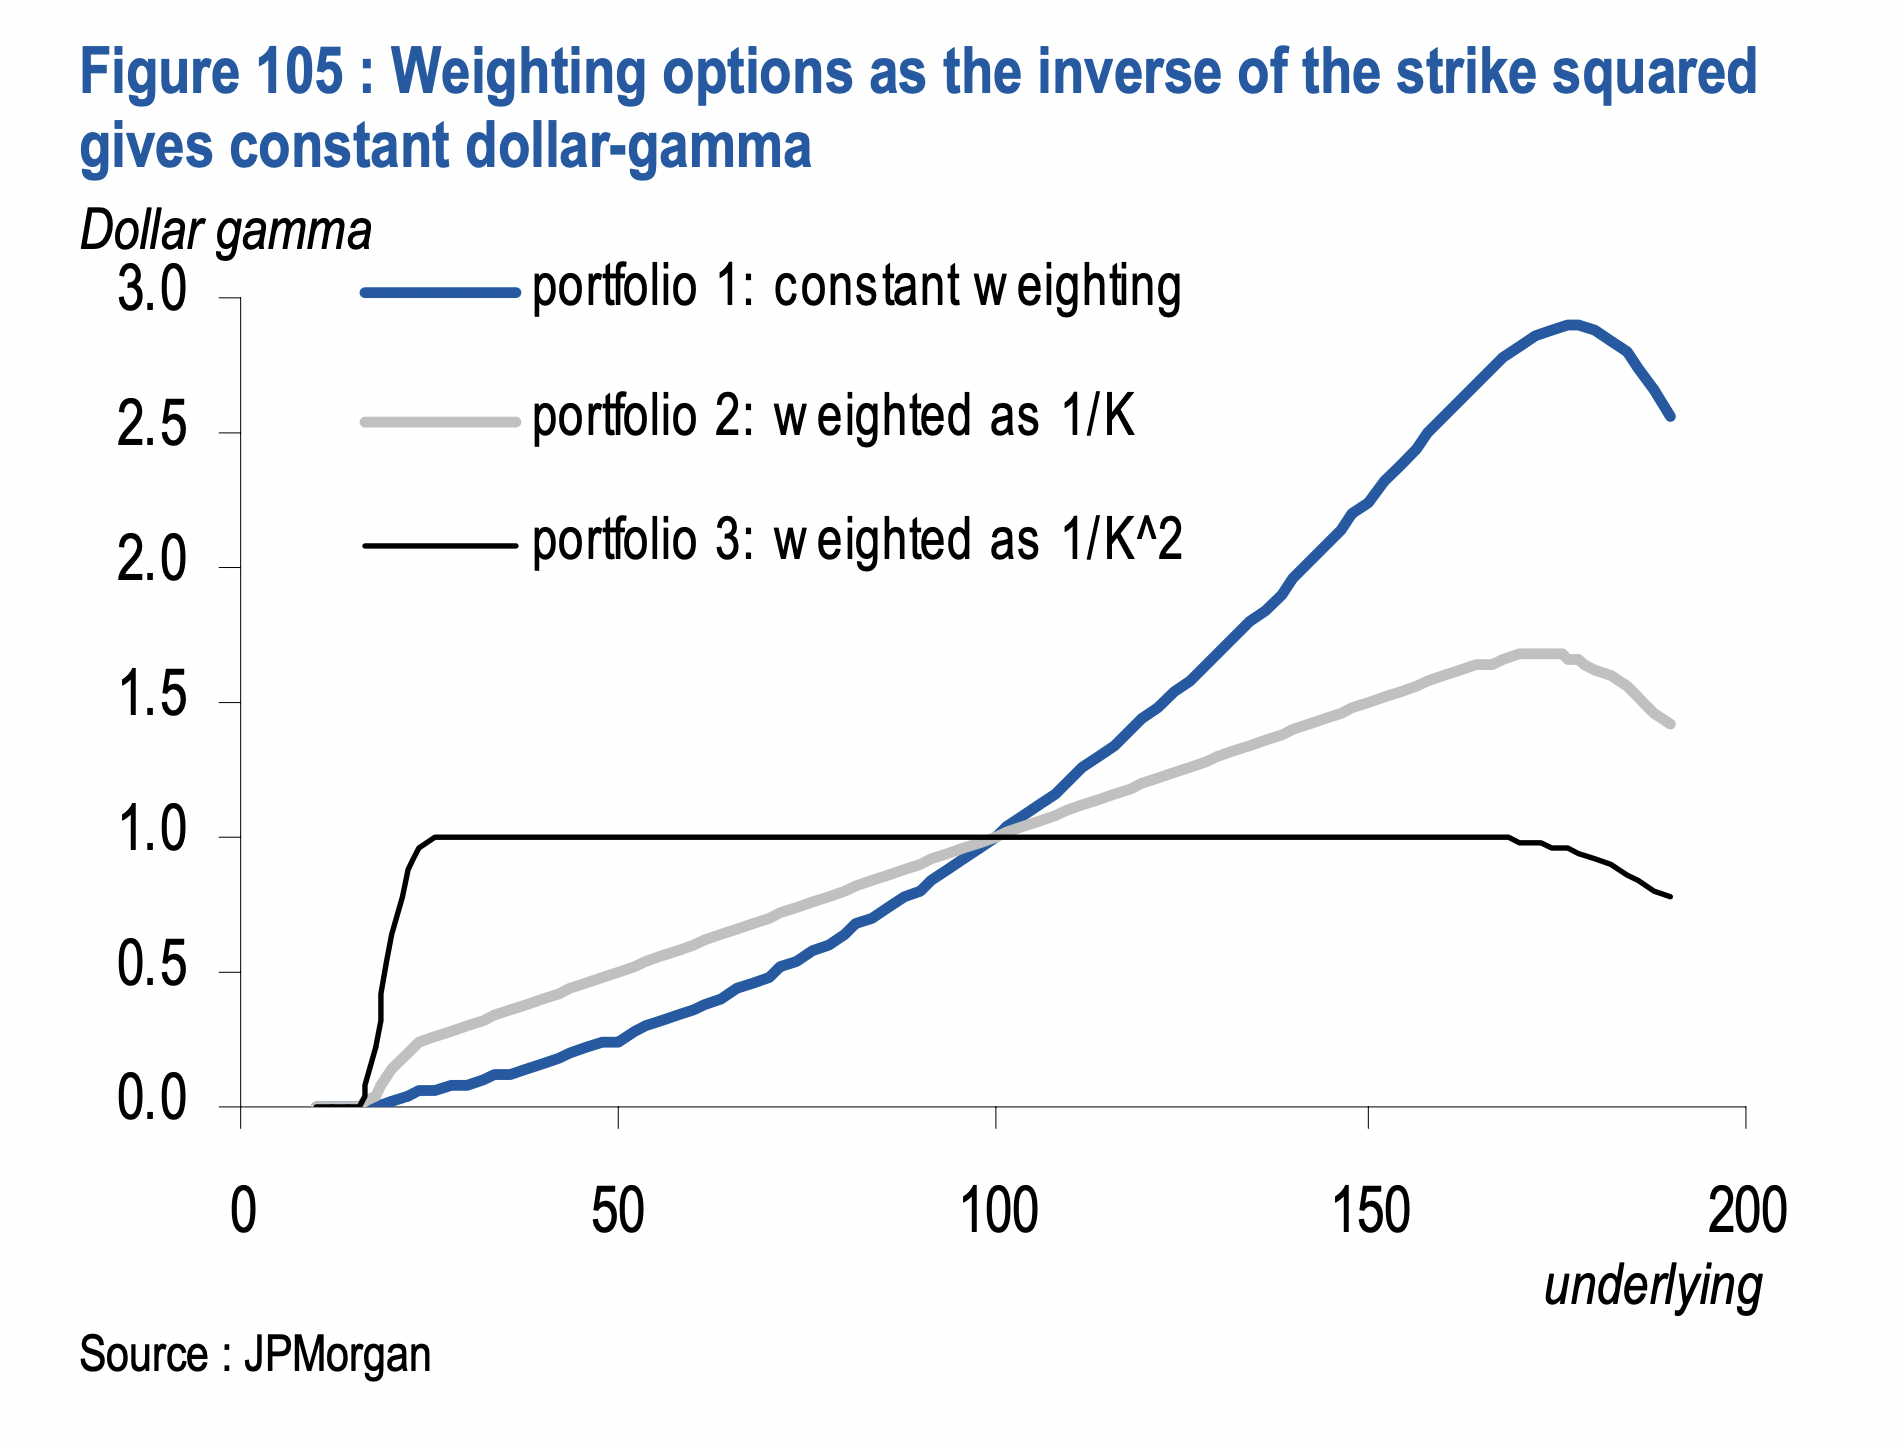
\includegraphics[width=0.65\textwidth]{include/img/jpm_varswap_gamma.png}
    \centering
    \caption{Dollar-gamma exposure for different swap flavours. Constant for variance swap, liner for gamma swap.}
    \label{fig:bivariate_contour}
\end{figure}

here the correct choice would be $f: x \mapsto x\log x - x$, which indeed yields the variable leg $\int_{0}^{T} \frac{S_t}{S_0} \sigma_t^2 dt$.

There exists some other flavours of swaps: corridor swaps, entropy swaps, correlation swaps, \textit{etc.} Volswaps are not really a thing as they cannot be statically replicated by a portfolio of options.

\subsubsection*{Extracting the forward variance curve}

Forward variance curve $\xi_0(\cdot)$ should be extracted from variance swap replication as a piece-wise constant c\`adl\`ag function, where each next level is built thanks to the SVI interpolation of the strip of calls and puts prices. The quantity $\xi_t(u)$ is the instantaneous variance at time $u > t$ seen from $t$.